\section{INTRODUCTION}
In recent years, extensive research has been conducted on Human-Drone Interaction (HDI) \cite{Tezza2019HDI-Survey}.
In particular, physical interaction between drones and humans has gained increasing attention, as it has the potential to expand the scope of drone applications \cite{Knierim2017virtual-reality-tactile-drones, Nitta2014hoverball}. 
However, ensuring physical and psychological safety during physical contact has been a significant challenge, especially when using conventional propeller-driven drones.  
The rapid rotation of propellers poses a potential risk of injury, making it difficult to design safe and natural interactions. 
Additionally, the high-frequency noise and mechanical appearance of propeller drones often induce psychological discomfort, further limiting their acceptance in close human proximity \cite{schaffer2021drone-noise-impact,Yeh2017Proxemics} .
To address these issues, previous studies have made proposals such as 
safeguard mechanisms to cover the drone body \cite{Atahi2017touch-based}, 
drones that has an familiar appearance to human \cite{Yeh2017Proxemics},
and bio-inspired propellers that make less noise \cite{noda2018development-of-low-noise-propeller}.

\begin{figure}
    \centering
    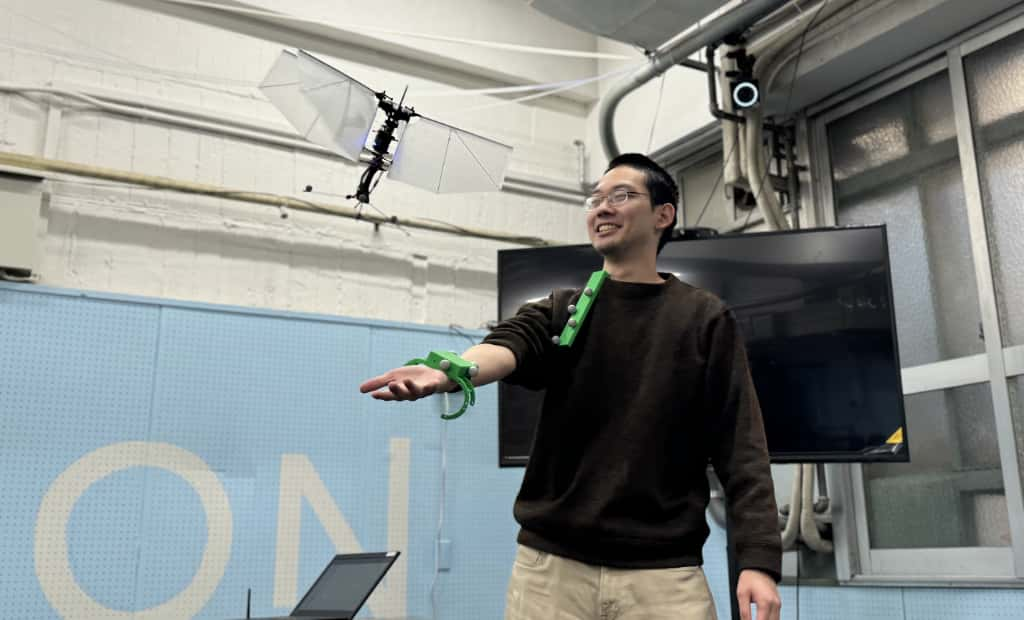
\includegraphics[width=\columnwidth]{falconer.jpg}
    \caption{Proposed falconer-like interaction system which takes human safety factors into account. 
    The flapping-wing drone approaches a human body following a planned path and performs a landing motion on a human palm.
    The human gesture system detects the position of the palm and the chest, and enables the user to stop the drone by bending the arm.}
    \label{fig:falconer}
\end{figure}

Similarly, flapping-wing drones, inspired by the flight of birds and insects, offer several inherent advantages that make them particularly suitable for physical interaction \cite{de2020flapping}.  
In contrast to propeller-driven drones, the soft and oscillatory motion of the wings minimizes the physical impact during contact, greatly enhancing physical safety.  
Second, flapping-wing drones produce more natural sound, reducing psychological discomfort during interaction.  
Third, the biomimetic appearance and motion of flapping-wing drones evoke a sense of familiarity, promoting more natural and engaging human-drone interaction.  
Despite these promising characteristics, most existing research on flapping-wing drones has been primarily focused on their mechanical characteristics such as aerodynamics, wing design, and flight control \cite{billingsley2021aerodynamic,rifai2008flapping-control,chin2020efficient-flapping}.
To the best of our knowledge, no prior study has specifically investigated the design of physical interaction system using flapping-wing drones.  
This presents a significant research gap in leveraging the unique properties of flapping-wing drones to enhance the quality of human-drone interaction.

To address this gap, it is essential to consider what type of interaction system would be suitable for flapping-wing drones.
One potential inspiration is falconry, a practice in which falconers guide birds of prey to land on their arms, which has a long history over centuries \cite{oggins2019falconry}.
In falconry, the falconer's arm serves as a dynamic landing platform for the bird.
This interaction model can be a cornerstone for designing a physical interaction system with flapping-wing drones as shown in Fig.~\ref{fig:falconer}, 
because it has the following versatile advantages:
\begin{enumerate}
    \item \textbf{Environment-adaptive interaction}\\  
    In crowded or spatially constrained environments, landing on a fixed surface is often impractical.  
    However, by utilizing the human body as a dynamic landing platform, the drone can overcome spatial limitations and operate more flexibly.  
    This approach is particularly useful in urban scenarios, public transportation, or greenhouses.
    \item \textbf{Personalized companion interaction}\\  
    By landing on a human palm, a drone can provide pet-like interaction, evoke emotional attachment, or facilitate social engagement.  
    This is particularly promising for children, the elderly, or individuals with social isolation, where physical interaction fosters a stronger sense of companionship.
\end{enumerate}
These advantages highlight the potential of falconer-like interaction as a key interaction modality for flapping-wing drones, enabling a wide range of applications in various scenarios.
Furthermore, if we only focus on the advantages of dynamic landing platform, we can simplify the mechanism of the perching motion of birds, which requires complex structures to realize as studied in the previous work \cite{roderick2021bird-inspired-perching},
by replacing perching with palm landing, which only requires a four-point contact between the drone and the human hand.

Therefore, in this study, we propose a falconer-like interaction system in which a flapping-wing drone performs a palm landing motion on a human hand, enabling direct physical contact in a safe manner.

To implement this system, we need to take into account two aspects of HDI:
\begin{enumerate}
    \item \textbf{Human gesture}\\
    Gestures for drone control should be intuitive and easy to understand for the user.
    Previous studies have proposed precise human gesture recognition systems based on algorithms such as deep learning \cite{guo2021hand-gesture-recognition} and hidden Markov models \cite{Wilson1999parametric-HMM}.
    However, these systems require complex models and setups, which are not suitable for applications for a sole simple purpose.
    Thus, we need to develop a simple and intuitive gesture system that can be easily implemented.
    \item \textbf{Drone trajectory planning}\\
    The trajectory planning of the drone should be designed to ensure physical and psychological safety during interaction.
    Previous studies have proposed trajectory planning methods for several purposes \cite{sandino2021object-detection-uncertainty, rezaee2024drones-collision-avoidance}.
    However, these methods are not directly applicable to the scenario of human interaction due to the lack of consideration of physical and psychological human safety factors.
    There has also been a study on the trajectory planning of drones for increasing the perceived safety of drones \cite{van2023perceived-safety}.
    Nevertheless, the study is mainly for avoiding the human body and not applicable to the physical interaction.
    Therefore, we need to design a trajectory planning method that considers both physical and psychological factors of human safety.
\end{enumerate}
Based on these considerations, we explain in detail how to design both the human gesture system and the drone trajectory planning system for the falconer-like interaction system in later sections.

The main contributions of this work can be summarized as
follows:
\begin{enumerate}
    \item We design a straight-forward detection system for human gestures that can be easily implemented.
    \item We design a trajectory planning method of drones that considers both physical and psychological factors of human safety.
    \item We demonstrate the feasibility of the proposed methods by real-world interaction experiments.
\end{enumerate}

The remainder of this paper is organized as follows. 
The basic mechanical characteristics and control method of flapping-wing drone is introduced in Section II. 
The human gesture system as an interface of the interaction system is described in Section III.
The motion planning based on physical and psychological factors is presented in Section IV,
followed by the experimental results in Section V before concluding in Section VI.